\documentclass{article}
\usepackage[x11names]{xcolor}
\usepackage{multirow}

% LNAI stuff

% TLP stuff

\usepackage{times}
% \usepackage{soul} % to strikeout, highline, etc.
\usepackage{url}
\usepackage[hidelinks]{hyperref}
\usepackage{graphicx}
\usepackage{booktabs}
\usepackage{algorithm}
\usepackage{algorithmic}
\urlstyle{same}
\usepackage[%textsize=tiny,
    prependcaption]{todonotes}
%

% OUR PACKAGES AND MACROS


\usepackage{tikz}
\tikzset{
    boxed/.style={draw, rectangle, rounded corners=4pt, fill=gray!10,inner sep=1em, anchor=center},
    event/.style={},
    smodel/.style={fill=gray!25},
    tchoice/.style={draw, circle},
    indep/.style={},
    proptc/.style = {-latex, dashed},
    propsm/.style = {-latex, thick},
    doubt/.style = {gray} }
\usetikzlibrary{calc, positioning, patterns, perspective}
%
\usepackage{hyperref}
\hypersetup{
    colorlinks=true,
    linkcolor=blue,
    citecolor=blue,
    urlcolor=blue, }
%
\usepackage{commath}

%\usepackage{ntheorem}
%\newtheorem{assumption}{Assumption}
\newtheorem{assumption}{Assumption}
\usepackage{amssymb}
\usepackage[normalem]{ulem}
% \usepackage[euler-digits,euler-hat-accent]{eulervm}
\usepackage[nice]{nicefrac}
\usepackage{stmaryrd}
\usepackage[smaller]{acronym}
\usepackage{multicol}
\usepackage{multirow}
\usepackage{cleveref}
\crefname{example}{ex.}{exs.}
\crefname{proposition}{prop.}{props.}
\crefname{assumption}{assumption}{assumptions}
\usepackage{hyphenat}
\hyphenation{
mo-dels mi-ti-ga-ted mi-ni-mal ex-am-ple spe-ci-fi-ca-tion
}
% Environments

\newtheorem{example}{Example}
\newtheorem{definition}{Definition}
\newtheorem{proposition}{Proposition}

% Commands

\def\tight{%
  \itemsep 0pt plus 1pt
  \parskip 0pt plus 1pt}

\newcommand{\ie}{\emph{i.e.}}
\newcommand{\eg}{\emph{e.g.}}
\newcommand{\eat}[1]{}
\newcommand{\at}[1]{\ensuremath{\!\del{#1}}}        %   argument
%
%   Notation
%
%   special sets
%
\newcommand{\cla}[1]{\ensuremath{{\mathcal{#1}}}}        %   class of something  
\newcommand{\clx}[1]{\ensuremath{{\mathbb{#1}}}}
%
%   connectives in logic programs
%
\newcommand{\conj}{\ensuremath{\wedge}} \newcommand{\disj}{\ensuremath{\vee}}
\newcommand{\clause}{\ensuremath{\leftarrow}}
\DeclareMathOperator{\naf}{\sim\!}
% \newcommand{\naf}{\ensuremath{\sim\!\!}}
\newcommand{\co}[1]{\ensuremath{\overline{#1}}}     %   complement
%\renewcommand{\complement}{\ensuremath{\complement \complement}}     %   complement
%
%   often used sets
%
\newcommand{\ATOMSset}{\ensuremath{\cla{A}}}
\newcommand{\Rset}{\ensuremath{\mathbb{R}}}
\newcommand{\LITERALSset}{\ensuremath{\cla{L}}}
\newcommand{\PATOMset}{\ensuremath{\ATOMSset_{\cla{P}}}}
\newcommand{\WATOMset}{\ensuremath{\ATOMSset_{\cla{W}}}}
\newcommand{\FACTSset}{\ensuremath{\cla{F}}}
\newcommand{\PROBFset}{\ensuremath{\cla{P}}}
\newcommand{\WEIGHTFset}{\ensuremath{\cla{W}}}
\newcommand{\RULESset}{\ensuremath{\cla{R}}}
\newcommand{\TCHOICEset}{\ensuremath{\cla{T}}}
\newcommand{\MODELset}{\ensuremath{\cla{M}}}
\newcommand{\EVENTSset}{\ensuremath{\cla{E}}}
\newcommand{\CONSISTset}{\ensuremath{\cla{C}}}
% \newcommand{\FRUITFUL}{\ensuremath{P_{\mathrm{fuitful}}}}
\newcommand{\SBF}{\ensuremath{P_{\sbf}}}
%
%   often used functions
%
%   error (loss)
\newcommand{\err}[1]{\ensuremath{\mathrm{err}\at{#1}}}
%
%   probability 
\newcommand{\prfunc}{\ensuremath{\mathrm{P}}}       
%   P(X = x)
\newcommand{\pr}[1]{\ensuremath{\prfunc\at{#1}}}    
%   P_X(x)
\newcommand{\prd}[1]{\ensuremath{\prfunc_{#1}}}     
\newcommand{\prT}{\prd{\TCHOICEset}}
\newcommand{\prM}{\prd{\MODELset}}
\newcommand{\prE}{\prd{\EVENTSset}}
\newcommand{\prC}{\prd{\cla{C}}}
%
%   weights 
\newcommand{\wgtfunc}{\ensuremath{\omega}}       
%   P(X = x)
\newcommand{\wgt}[1]{\ensuremath{\wgtfunc\at{#1}}}    
%   P_X(x)
\newcommand{\wgtd}[1]{\ensuremath{\wgtfunc_{#1}}}     
\newcommand{\wgtT}{\wgtd{\TCHOICEset}}
\newcommand{\wgtM}{\wgtd{\MODELset}}
\newcommand{\wgtE}{\wgtd{\EVENTSset}}
\newcommand{\wgtC}{\wgtd{\cla{R}}}
\newcommand{\wgte}[1]{\ensuremath{\wgtE\at{#1}}}
\newcommand{\wgtm}[1]{\ensuremath{\wgtM\at{#1}}}
\newcommand{\wgtt}[1]{\ensuremath{\wgtT\at{#1}}}
\newcommand{\wgtc}[1]{\ensuremath{\wgtC\at{#1}}}
%
%   local notation
%
 %   m(x)
\newcommand{\pw}[1]{\ensuremath{\mu\at{#1}}}           
%   m_T     total choices 
\newcommand{\pwT}{\ensuremath{\mu_{\TCHOICEset}}}   
%   m_T(x)
\newcommand{\pwt}[1]{\ensuremath{\pwT\at{#1}}}     
%   m_M     stable models  
\newcommand{\pwM}{\ensuremath{\mu_{\MODELset}}}   
%   m_M(x)
\newcommand{\pwm}[1]{\ensuremath{\pwM\at{#1}}}     
%   m_C     eq. classes 
\newcommand{\pwC}{\ensuremath{\mu_{\textrm{\cla{C}}}}}   
%   m_C(x)
\newcommand{\pwc}[1]{\ensuremath{\pwC\at{#1}}}     
%   m_E     events 
\newcommand{\pwE}{\ensuremath{\mu_{\EVENTSset}}}   
%   m_E(x)
\newcommand{\pwe}[1]{\ensuremath{\pwE\at{#1}}}     
%
%
%
\newcommand{\stablecore}[1]{\ensuremath{\left\llbracket #1 \right\rrbracket}}
\newcommand{\inconsistent}{\bot}
\newcommand{\given}{\ensuremath{~\middle|~}}
\newcommand{\consequenceclass}{\ensuremath{\Lambda}}
\newcommand{\indepclass}{\ensuremath{\Diamond}}
\newcommand{\probfact}[2]{\ensuremath{#1:#2}}
\newcommand{\probrule}[3]{\probfact{#1}{#2} \leftarrow #3}
\newcommand{\weightfact}[2]{\ensuremath{#1:#2}}
\newcommand{\weightrule}[3]{\weightfact{#1}{#2} \leftarrow #3}
\newcommand{\class}[1]{\ensuremath{[{#1}]_{\sim}}}
\newcommand{\tcgen}[1]{\MODELset\at{#1}}
\newcommand{\condsymb}[2]{\ensuremath{p_{#1|#2}}}
\newcommand{\lpmln}{\texttt{LP\textsuperscript{MLN}}}
\newcommand{\emptyevent}{\ensuremath{\lambda}}
% \newcommand{\powerset}[1]{\ensuremath{\mathbb{P}\at{#1}}}
\newcommand{\powerset}[1]{\ensuremath{\mathrm{2}^{#1}}}
%
%   Acronyms
%
\acrodef{BK}[BK]{background knowledge}
\acrodef{ASP}[ASP]{answer set program}
% \acrodef{ASP}[ASP]{answer set prolog}
\acrodef{NP}[NP]{normal program}
\acrodef{DP}[DP]{disjunctive program}
\acrodef{LP}[LP]{logic program}
\acrodef{PCR}[PCR]{program with choice rules}
\acrodef{DS}[DS]{distribution semantics}
\acrodef{PF}[PF]{probabilistic fact}
\acrodef{WF}[WF]{weighted fact}
\acrodef{TC}[TC]{total choice}
\acrodef{SM}[SM]{stable model}
\acrodef{SC}[SC]{stable core}
\acrodef{KL}[KL]{Kullback-Leibler}
\acrodef{SBF}[SBF]{simple but fruitful}
\acrodef{RSL}[RSL]{random set of literals}
\acrodef{RCE}[RCE]{random consistent event}
\acrodef{SASP}[SASP]{stochastic answer set program}
\acrodef{WASP}[WASP]{weighted answer set program}
\acrodef{HMM}[HMM]{hidden Markov model}
\acrodef{MAP}[MAP]{maximum a posteriori}
\acrodef{MLE}[MLE]{maximum likelihood estimation}
\acrodef{BI}[BI]{Bayesian inference}
\acrodef{PLP}[PLP]{probabilistic logic programming}
%
%   Common objects
%
\newcommand{\sbf}{\ensuremath{\mathrm{1}}}
%
%   Reviewing
%
\newcounter{revcounter}
\newcommand{\LOOK}{\ensuremath{\blacksquare}}
\newcommand{\delete}[1]{\sout{#1}}
\newcommand{\sidenote}[1]{\stepcounter{revcounter}{\color{red!50!black}\(\vert^{\arabic{revcounter}}\)}\marginpar{{\color{red!50!black}\(^{\arabic{revcounter}}\vert\)}\scriptsize #1}}
\newcommand{\defnote}[1]{\marginpar{\scriptsize{{\color{blue!50!black}\bf def.~}#1}}}
\newcommand{\topicnote}[1]{{\scriptsize\color{red!50!black}$\blacktriangleright$}\marginpar{\scriptsize{\color{red!50!black}\it #1}}}
\newcommand{\replace}[2]{\delete{#1}\sidenote{#2}}
\newcommand{\franc}[1]{{\color{green!30!black}#1}}
\newcommand{\bruno}{\color{red!60!black}}
%\newcommand{\spa}[1]{{\color{brown!80!black}{#1}}}
\newcommand{\dietmar}[1]{{\color{brown!40!black}#1}}

% -- side notes --

\newcommand{\selfnote}[1]{\todo[backgroundcolor=green!20]{{\footnotesize #1}}}
\newcommand{\spanote}[1]{{\todo[size=footnotesize,color=teal!20]{\textbf{SPA:} #1}}}
\newcommand{\dsnote}[1]{{\todo[size=footnotesize,color=teal!20]{\textbf{DS:} #1}}}
\newcommand{\francnote}[1]{{\todo[size=footnotesize,color=green!30]{\textbf{FC:} #1}}}
\newcommand{\bdnote}[1]{{\todo[size=footnotesize,color=red!60]{\textbf{BD:} #1}}}

\usepackage{natbib}
\renewcommand{\cite}{\citep}

\begin{document}

%   PREAMBLE / METADATA

\title{%
	Examples for ``An Algebraic Approach to Stochastic
	Answer~Set~Programming''
}
\author{%
	Francisco Coelho
	\and
	Bruno Dinis
	\and %
	Dietmar Seipel
	\and %
	Salvador Abreu   %
}
% \institute{%
%     University of Évora \\
%     \email{\{fc,bruno.dinis,spa\}@uevora.pt} \and
%     NOVA LINCS \and
%     CIMA \and
%     Universit\"at W\"urzburg \\
%     \email{dietmar.seipel@uni-wuerzburg.de}
% }

\maketitle

\begin{abstract}
	We address the problem of propagating the probabilities from the     annotated facts of an \acl{ASP} to its \aclp{SM}, and from there to     general events in the program's domain.
	% 
	Our approach is algebraic in the sense that it relies on an
	equivalence relation over the set of events, and uncertainty is
	expressed with variables and polynomial expressions.
	% 
	We propagate probability in the space of models and events, instead
	of dealing with the syntax of the program.
	% 
	We illustrate our methods with two examples, one of which shows a
	connection to bayesian networks.
\end{abstract}

\begin{quotation}
	\textbf{Keywords:} Answer-Set Programming, Stable Models, Probabilistic Logic Programming
\end{quotation}

\section{A Simple but Fruitful Example}

Consider \(A\) to be the following \ac{SASP}:
\begin{equation}\label{eq:fruitful}
	\begin{split}
		\probfact{a&}{0.3}, \\
		b \vee c          & \clause a
	\end{split}
\end{equation}
which has the set \({\cal P} = \{ a:0.3 \}\) of probabilistic
facts.  This program is transformed into the disjunctive logic
program
\begin{equation}\label{eq:derived.fruitful}
	\begin{split}
		a \vee \co{a},\\
		b \vee c          & \clause a,
	\end{split}
\end{equation}
with the set
\( {\cal M} = \{\, \co{a}, ab, ac\, \} \)
of three stable models.
We use short-hand expressions like \(ab\) to denote a set
of literals such as \(\set{a, b}\).

Consider the program
\begin{equation*}
	\begin{split}
		\probfact{a&}{0.3}, \\
		b & \clause a
	\end{split}
\end{equation*}
We don't follow the clause \(b \clause a\) to attribute a probability to \(b\). Instead, that will result from considering how events are related with the \aclp{SM} and these with the \aclp{TC}. If one follows the steps of \cref{sec:propagating.probalilities} would get
\begin{equation*}
	\begin{split}
		\prE\at{a} & = \prE\at{b} = \prE\at{ab} = 0.05,\\
		\prE\at{\co{a}} & = \prE\at{\co{a} b} = \prE\at{\co{a}\co{b}} = \frac{7}{60},\\
		\prE\at{\set{}} & = 0.5.\\
	\end{split}
\end{equation*}

The atoms of program \cref{eq:fruitful} are
\(\ATOMSset = \set{a, b, c}\) and the literals are
\begin{equation*}
	\LITERALSset = \set{\, \co{a}, \co{b}, \co{c}, a, b, c\, }.
\end{equation*}
In this case, \(\EVENTSset\) has \(2^6 = 64\) elements.  Some, such as
\(\set{\co{a}, a, b}\), contain an atom and its negation (\(a\) and
\(\co{a}\) in that case) and are inconsistent.  The set of atoms
\(\ATOMSset = \set{a, b, c}\) above generates \(37\) inconsistent
events and \(27\) consistent events.  Notice that the empty set is an
event, that we denote by \emptyevent.

As above, to simplify notation we write events as \(\co{a}ab\) instead
of \(\set{\co{a}, a, b}\).

Consider the program $B$ defined by
\begin{equation*}
	\begin{split}
		\probfact{a&}{0.3},\\
		\probfact{b&}{0.6},\\
		c & \clause a \wedge b.
	\end{split}\label{eq:total.choices}
\end{equation*}
The probabilistic facts of \(B\) are
\[ \PROBFset_{B} = \set{~\probfact{a}{0.3}, \probfact{b}{0.6}~}, \]
and the total choices are
\[ \TCHOICEset_{B} = \set[2]{\:
		\set[1]{a, b},
		\set[1]{a, \co{b}},
		\set[1]{\co{a}, b},
		\set[1]{\co{a}, \co{b}}\: }. \]
E.g., the total choice \(\set{\co{a}, b} \)
results from choosing \(a' = \co{a}\) from the probabilistic fact
$\probfact{a}{0.3}$ and $b' = b$ from \(\probfact{b}{0.6}, \)
while \(\set{a, b} \) results from choosing \(a' = a\) from
\(\probfact{a}{0.3}\) and \(b' = b\) from \(\probfact{b}{0.6}\).

Continuing with the program from \cref{eq:fruitful}, the
probabilities of the \aclp{TC} are:
\begin{equation*}
	\begin{aligned}
		\prT\at{\set[1]{a, b}}           & = 0.3 \times 0.6           &                  & = 0.18, \\
		\prT\at{\set[1]{a, \co{b}}}      & = 0.3 \times \co{0.6}      & = 0.3 \times 0.4 & = 0.12, \\
		\prT\at{\set[1]{\co{a}, b}}      & = \co{0.3} \times 0.6      & = 0.7 \times 0.6 & = 0.42, \\
		\prT\at{\set[1]{\co{a}, \co{b}}} & = \co{0.3} \times \co{0.6} & = 0.7 \times 0.4 & = 0.28.
	\end{aligned}
\end{equation*}

Suppose that in this program we change the probability in
\(\probfact{b}{0.6}\) to \(\probfact{b}{1.0}\).  Then the \aclp{TC}
are the same but the probabilities become
\begin{equation*}
	\begin{aligned}
		\prT\at{\set[1]{a, b}}           & = 0.3 \times 1.0           &                  & = 0.3, \\
		\prT\at{\set[1]{a, \co{b}}}      & = 0.3 \times \co{1.0}      & = 0.3 \times 0.0 & = 0.0, \\
		\prT\at{\set[1]{\co{a}, b}}      & = \co{0.3} \times 1.0      & = 0.7 \times 1.0 & = 0.7, \\
		\prT\at{\set[1]{\co{a}, \co{b}}} & = \co{0.3} \times \co{1.0} & = 0.7 \times 0.0 & = 0.0.
	\end{aligned}
\end{equation*}
which, as expected from stating that \(\probfact{b}{1.0}\), is like
having \(b\) as a (deterministic) fact:
\begin{equation*}
	\begin{split}
		\probfact{a&}{0.3}, \\
		b &, \\
		c & \clause a \wedge b.
	\end{split}
\end{equation*}

Continuing the study of the program \cref{eq:fruitful}, the \acl{TC} \(t = \set{\co{a}}\)
entails a single \acl{SM}, \(\co{a}\), so
\( \MODELset\at{\set{\co{a}}} = \set{\co{a}} \) and, for
\(t = \set{a}\), the program has two \aclp{SM}:
\( \MODELset\at{\set{a}} = \set{ab, ac}\).

\begin{equation*}
	\begin{array}{l|r}
		t \in \TCHOICEset   & \MODELset\at{t} \\
		\hline \set{\co{a}} & \co{a}          \\
		\set{a}             & ab, ac
	\end{array}
\end{equation*}
The second case illustrates that propagating probabilities from
\aclp{TC} to \aclp{SM} entails a non-deterministic step: \textit{How
	to propagate the probability \(\prT\at{\set{a}}\) to each one of
	the \aclp{SM} \(ab\) and \(ac\)?}

As a first step to propagate probability from \aclp{TC} to
events, consider a possible
propagation of \(\prT:\TCHOICEset \to \intcc{0,1}\) from \aclp{TC}
to the \aclp{SM}, \(\prM:\MODELset \to \intcc{0,1}\).

The \aclp{SM} are the ones from its derived program (in
\cref{eq:derived.fruitful}):
\[ \MODELset = \set{\co{a}, ab, ac}. \]
It might seem straightforward to assume \(\prM\at{\co{a}}=0.7\) but
\emph{there is no explicit way to assign values to \(\prM\at{ab}\) and
	\(\prM\at{ac}\)}.  Instead, we assume this lack of information and use a
parameter \(\theta\) as in
\begin{equation*}
	\begin{aligned}
		\prM\at{ab} & = 0.3\, \theta, \\
		\prM\at{ac} & = 0.3\, (1 - \theta)
	\end{aligned}
\end{equation*}
to express our knowledge that $ab$ and $ac$ are models related in a
certain way and, simultaneously, our uncertainty about that
relation.  In general, there might be necessary several such
parameters, each associated to a \acl{SM} \(s\) and a \acl{TC}
\(t\), so we write \(\theta=\theta_{s,t}\).

A value for \(\theta_{s,t}\) can't be determined just with the
information given in that program, but might be estimated with the
help of further information, such as empirical distributions from
datasets.

\begin{figure}[t]
	\begin{center}
		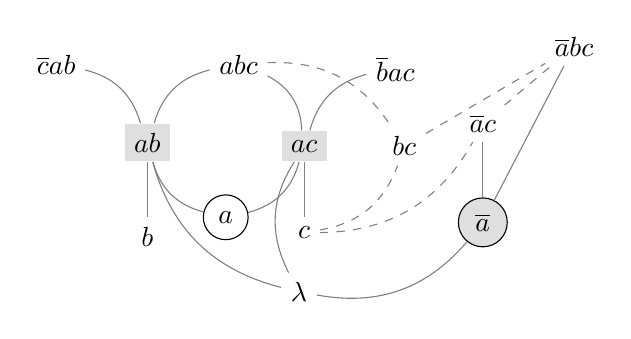
\begin{tikzpicture}[node distance=2em]
			\node[event] (E) {\(\emptyevent\)};
			\node[tchoice, above left = of E] (a) {\(a\)};
			\node[smodel, above left = of a] (ab) {\(ab\)};
			\node[smodel, above right = of a] (ac) {\(ac\)};
			\node[event, below = of ab] (b) {\(b\)};
			\node[event, below = of ac] (c) {\(c\)};
			\node[event, above right = of ab] (abc) {\(abc\)};
			\node[event, above left = of ab] (abC) {\(\co{c}ab\)};
			\node[event, above right = of ac] (aBc) {\(\co{b}ac\)};
			\node[indep, right = of ac] (bc) {\(bc\)};
			\node[tchoice, smodel, below right = of bc] (A) {\(\co{a}\)};
			\node[event, above = of A] (Ac) {\(\co{a}c\)};
			\node[event, above right = of Ac] (Abc) {\(\co{a}bc\)};
			% ----
			\draw[doubt] (a) to[bend left] (ab);
			\draw[doubt] (a) to[bend right] (ac);

			\draw[doubt] (ab) to[bend left] (abc);
			\draw[doubt] (ab) to[bend right] (abC);

			\draw[doubt] (ac) to[bend right] (abc);
			\draw[doubt] (ac) to[bend left] (aBc);

			\draw[doubt, dashed] (Ac) to (Abc);

			\draw[doubt] (A) to (Ac);
			\draw[doubt] (A) to (Abc);

			\draw[doubt] (ab) to[bend right] (E);
			\draw[doubt] (ac) to[bend right] (E);
			\draw[doubt] (A) to[bend left] (E);

			\draw[doubt] (ab) to (b);
			\draw[doubt] (ac) to (c);
			
			\draw[doubt, dashed] (c) to[bend right] (bc);
			\draw[doubt, dashed] (abc) to[bend left] (bc);
			\draw[doubt, dashed] (bc) to (Abc);
			\draw[doubt, dashed] (c) to[bend right] (Ac);
		\end{tikzpicture}
	\end{center}

	\caption{%
		This (partial sub-/super-set) diagram shows some events related to
		the \aclp{SM} of the program \cref{eq:fruitful}.  The circle nodes
		are \aclp{TC} and shaded nodes are \aclp{SM}.  Solid lines
		represent relations with the \aclp{SM} and dashed lines some
		sub-/super-set relations with other events.  The set of events
		contained in all \aclp{SM}, denoted by \(\bottomclass\), is
		\(\set{ \emptyevent }\) in this example, because
		\(\co{a} \cap ab \cap ac = \emptyset = \emptyevent\).}
	\label{fig:running.example}
\end{figure}

\begin{figure}[t]
	\begin{center}
		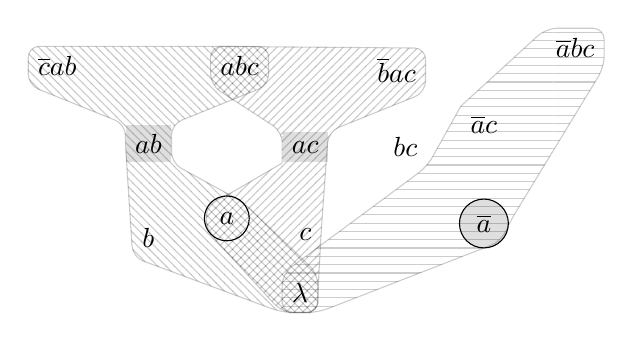
\begin{tikzpicture}[node distance=2em]
			\node[event] (E) {\(\emptyevent\)};
			\node[tchoice, above left = of E] (a) {\(a\)};
			\node[smodel, above left = of a] (ab) {\(ab\)};
			\node[smodel, above right = of a] (ac) {\(ac\)};
			\node[event, below = of ab] (b) {\(b\)};
			\node[event, below = of ac] (c) {\(c\)};
			\node[event, above right = of ab] (abc) {\(abc\)};
			\node[event, above left = of ab] (abC) {\(\co{c}ab\)};
			\node[event, above right = of ac] (aBc) {\(\co{b}ac\)};
			\node[indep, right = of ac] (bc) {\(bc\)};
			\node[tchoice, smodel, below right = of bc] (A) {\(\co{a}\)};
			\node[event, above = of A] (Ac) {\(\co{a}c\)};
			\node[event, above right = of Ac] (Abc) {\(\co{a}bc\)};
			% ----
			\path[draw, rounded corners, pattern=north west lines, opacity=0.2]
			(ab.west) -- (ab.north west) --
			% 
			(abC.south west) -- (abC.north west) -- (abC.north) --
			% 
			(abc.north east) -- (abc.east) -- (abc.south east) --
			% 
			(ab.north east) -- (ab.east) -- (ab.south east) --
			% 
			(a.north east) --
			% 
			(E.north east) -- (E.east) --
			(E.south east) -- (E.south) --
			(E.south west) --
			% 
			(b.south west) --
			% 
			(ab.west) ;
			% ----
			\path[draw, rounded corners, pattern=north east lines, opacity=0.2]
			(ac.south west) -- (ac.west) -- (ac.north west) --
			% 
			(abc.south west) -- (abc.west) -- (abc.north west) --
			% 
			(aBc.north east) -- (aBc.east) -- (aBc.south east) --
			% 
			(ac.north east) --
			% 
			(c.east) --
			% 
			(E.east) -- (E.south east) -- (E.south) -- (E.south west) --
			% 
			(a.south west) -- (a.west) -- (a.north west) -- (a.north) --
			% 
			(ac.south west) ;
			% ----
			\path[draw, rounded corners, pattern=horizontal lines, opacity=0.2]
			% (A.north west) --
			% 
			(Ac.north west) --
			% 
			(Abc.north west) -- (Abc.north) --
			(Abc.north east) -- (Abc.south east) --
			% 
			% (Ac.north east) -- (Ac.east) --
			% 
			(A.east) -- (A.south east) --
			% 
			(E.south east) -- (E.south) --
			(E.south west) -- (E.west) --
			(E.north west) --
			% 
			(bc.south east) --
			% 
			(Ac.north west) ;
		\end{tikzpicture}
	\end{center}

	\caption{Classes of (consistent) events related to the \aclp{SM} of
		\cref{eq:fruitful} are defined through sub-/super-set relations.
		In this picture we can see, for example, that
		\(\set{\co{c}ab, ab, b}\) and \(\set{a, abc}\) are part of
		different classes, represented by different fillings.  As before,
		the circle nodes are \aclp{TC} and shaded nodes are \aclp{SM}.
		Notice that \(bc\) is not in a shaded area.}
	\label{fig:running.example.classes}
\end{figure}

\begin{figure}[t]
	\begin{center}
		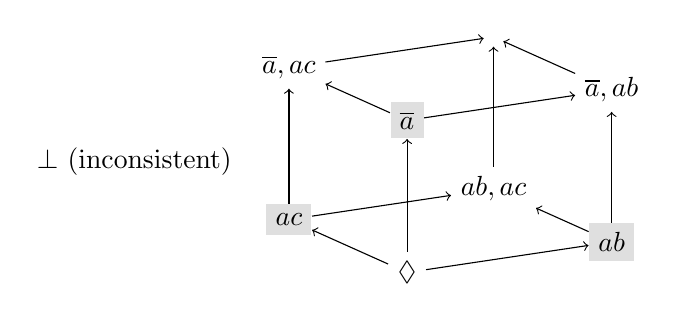
\begin{tikzpicture}[3d view]
			\node[event] (INDEPENDENT) at (0,0,0){\(\indepclass\)};
			\node[smodel] (A) at (0,0,2) {\(\co{a}\)};
			\node[smodel] (ab) at (3,0,0) {\(ab\)};
			\node[smodel] (ac) at (0,3,0) {\(ac\)};
			\node[event] (Aab) at (3,0,2) {\(\co{a},ab\)};
			\node[event] (Aac) at (0,3,2) {\(\co{a},ac\)};
			\node[event] (abac) at (3,3,0) {\(ab,ac\)};
			\node[event] (Aabac) at (3,3,2) {\(\bottomclass\)};
			\node[event] (INCONSISTENT) at (-4, 0, 2) {\(\inconsistent\)
				(inconsistent)};
			% ----
			\draw[->] (INDEPENDENT) -- (A);
			\draw[->] (INDEPENDENT) -- (ab);
			\draw[->] (INDEPENDENT) -- (ac);
			\draw[->] (A) -- (Aab);
			\draw[->] (A) -- (Aac);
			\draw[->] (ab) -- (Aab);
			\draw[->] (ab) -- (abac);
			\draw[->] (ac) -- (Aac);
			\draw[->] (ac) -- (abac);
			\draw[->] (Aab) -- (Aabac);
			\draw[->] (Aac) -- (Aabac);
			\draw[->] (abac) -- (Aabac);
		\end{tikzpicture}
	\end{center}

	\caption{%
		Lattice of the \aclp{SC} from \cref{eq:fruitful}.  In this diagram
		the nodes are the different \aclp{SC} that result from the
		\aclp{SM} plus the \emph{inconsistent} class (\(\inconsistent\)).
		The bottom node (\(\indepclass\)) is the class of
		\emph{independent} events, those that have no sub-/super-set
		relation with the \acp{SM} and the top node (\(\bottomclass\))
		represents events related with all the \acp{SM}.  As in previous
		diagrams, shaded nodes represent the \acp{SM}.}
	\label{fig:fruitful.lattice}
\end{figure}

Continuing \cref{eq:fruitful}, depicted in
\cref{fig:running.example,fig:running.example.classes,fig:fruitful.lattice},
and \(\MODELset = \set{ab, ac, \co{a}}\), consider the following
\aclp{SC} of some events:
\begin{equation*}
	\begin{aligned}
		\stablecore{a}           & = \set{s \in \MODELset \given s \subseteq a \vee a \subseteq s}                                        & = \set{ab, ac} \\
		\stablecore{abc}         & = \set{s \in \MODELset \given s \subseteq abc \vee abc \subseteq s}                                    & = \set{ab, ac} \\
		\stablecore{\co{c}ab}    & = \set{s \in \MODELset \given s \subseteq \co{c}ab \vee \co{c}ab \subseteq s}                          & = \set{ab}     \\
		\stablecore{bc}          & = \set{s \in \MODELset \given s \subseteq bc \vee bc \subseteq s}                                      & = \emptyset    \\
		\stablecore{\emptyevent} & = \set{s \in \MODELset \given s \subseteq \emptyset \vee \emptyset \subseteq s} = \set{ab, ac, \co{a}} & = \bottomclass \\
	\end{aligned}
\end{equation*}
Events \(a\) and \(abc\) have the same \ac{SC}, while \(\co{c}ab\) has
a different \ac{SC}.  Also, \(bc\) is \emph{independent of}
(\emph{i.e.}\ not related to) any \acl{SM}.  Since events are sets of
literals, the empty set is an event and a subset of any \ac{SM}.

Consider again \cref{eq:fruitful}.  As previously stated, the
\aclp{SM} are the elements of \(\MODELset = \set{\co{a}, ab, ac}\)
so the quotient set of this relation is
\begin{equation*}
	\class{\EVENTSset} = \set{
		\begin{array}{lll}
			\inconsistent,           &
			\indepclass,             &
			\stablecore{\co{a}},       \\
			\stablecore{ab},         &
			\stablecore{ac},         &
			\stablecore{\co{a}, ab},   \\
			\stablecore{\co{a}, ac}, &
			\stablecore{ab, ac},     &
			\bottomclass
		\end{array}
	},
\end{equation*}
where \(\indepclass\) denotes the class of \emph{independent
	events} \(e\) such that \(\stablecore{e} = \set{\emptyset}\),
while \(\bottomclass = \stablecore{\MODELset}\) is the set of
events related with all \acp{SM}.  We have:
%\note{Remark the odd nature of \(\bottomclass\).} EDIT:fc fix columns width
%
\begin{equation*}
	\begin{array}{l|lr}
		\stablecore{e}
		 & \class{e}
		 & \# \class{e}                                                                       \\
		\hline
		%
		\inconsistent
		 & \co{a}a, \ldots
		 & 37                                                                                 \\
		%
		\indepclass
		 & \co{b}, \co{c}, bc, \co{b}a, \co{b}c, \co{bc}, \co{c}a, \co{c}b, \co{bc}a
		 & 9                                                                                  \\
		%
		\co{a}
		 & \co{a}, \co{a}b, \co{a}c, \co{ab}, \co{ac}, \co{a}bc, \co{ac}b, \co{ab}c, \co{abc}
		 & 9                                                                                  \\
		%
		ab
		 & b, ab, \co{c}ab
		 & 3                                                                                  \\
		%
		ac
		 & c, ac, \co{b}ac
		 & 3                                                                                  \\
		%
		\co{a}, ab
		 &
		 & 0                                                                                  \\
		%
		\co{a}, ac
		 &
		 & 0
		%
		\\
		%
		ab, ac
		 & a, abc
		 & 2                                                                                  \\
		%
		\bottomclass
		 & \emptyevent
		 & 1
		\\
		%
		\hline \class{\EVENTSset}
		 & \EVENTSset
		 & 64
	\end{array}
\end{equation*}

Notice that \(bc \in \indepclass\), as hinted by
\cref{fig:running.example,fig:running.example.classes}.

The program from \cref{eq:fruitful} has no information about the
probabilities of the \aclp{SM} that result from the \acl{TC}
\(t = \set{a}\).  These models are
\(\MODELset\at{\set{a}} = \set{ab, ac}\) so we need two
parameters
\(\theta_{ab, \set{a}}, \theta_{ac, \set{a}} \in \intcc{0,1}\)
and such that

\begin{equation*}
	\theta_{ab, \set{a}} + \theta_{ac, \set{a}} = 1.
\end{equation*}
If we let \(\theta = \theta_{ab, \set{a}}\) then
\begin{equation*}
	\theta_{ac, \set{a}} = 1 - \theta = \co{\theta}.
\end{equation*}
Also
\begin{equation*}
	\begin{split}
		\theta_{ab, \set{\co{a}}} &= 0,\\
		\theta_{ac, \set{\co{a}}} &= 0
	\end{split}
\end{equation*}
because \(ab, ac \not\in\MODELset\at{\co{a}}\).

\begin{equation*}
	\begin{array}{c||l|ccc|ccc|c|c|r}
		%=====================================================
		  &
		A & B                                         & C      & D           & E & F & G & H & I & J
		\\[3pt]
		\hline
		\hline
		\multirow{3}{*}{\phantom{2em}}
		  & \multirow{3}{*}{\stablecore{e}}
		  & \multicolumn{3}{c|}{\pwm{s,\set{\co{a}}}}
		  & \multicolumn{3}{c|}{\pwm{s,\set{a}}}
		  & \pwc{\class{e},\set{\co{a}}}
		  & \pwc{\class{e},\set{a}}
		%  & \multicolumn{3}{c|}{\pwm{s, \co{a}}}
		%  & \multicolumn{3}{c|}{\pwm{s, a}}
		%  & \pwc{\class{e}, \co{a}}
		%  & \pwc{\class{e}, a}
		  & \multirow{3}{*}{\pwc{\class{e}}}
		\\[2pt]
		%=====================================================
		  &
		  & \co{a}                                    & ab     & ac
		  & \co{a}                                    & ab     & ac
		  & \pwt{\set{\co{a}}}
		  & \pwt{\set{a}}
		  &
		\\[2pt]
		%=====================================================
		  &
		  & 1                                         & 0      & 0
		  & 0                                         & \theta & \co{\theta}
		  & 0.7
		  & 0.3
		  &
		\\[3pt]
		%=====================================================
		\hline
		1
		  & \co{a}
		% & \boxed{1}                           & 0              & 0
		% & \boxed{0}                           & \theta         & \co{\theta}
		  & 1                                         &        &
		  & 0                                         &        &
		  & 1
		  & 0
		  & 0.7
		\\[2pt]
		%=====================================================
		%
		2
		  & ab
		  &                                           & 0      &
		  &                                           & \theta &
		  & 0
		  & \theta
		  & 0.3\theta
		\\[2pt]
		%=====================================================
		%
		3
		  & ac
		  &                                           &        & 0
		  &                                           &        & \co{\theta}
		  & 0
		  & \co{\theta}
		  & 0.3\co{\theta}
		\\[2pt]
		%=====================================================
		%
		4
		  & \co{a}, ab
		  & 1                                         & 0      &
		  & 0                                         & \theta &
		  & 1
		  & \theta
		  & 0.7 + 0.3\theta
		\\[2pt]
		%=====================================================
		%
		5
		  & \co{a}, ac
		  & 1                                         &        & 0
		  & 0                                         &        & \co{\theta}
		  & 1
		  & \co{\theta}
		  & 0.7 + 0.3\co{\theta}
		\\[2pt]
		%=====================================================
		%
		6
		  & ab, ac
		  &                                           & 0      & 0
		  &                                           & \theta & \co{\theta}
		  & 0
		  & \theta + \co{\theta} = 1
		  & 0.3
		\\[2pt]
		%=====================================================
		%
		7
		  & \bottomclass
		  & 1                                         & 0      & 0
		  & 0                                         & \theta & \co{\theta}
		  & 1
		  & \theta + \co{\theta} = 1
		  & 1
		%=====================================================
	\end{array}
\end{equation*}

Continuing \cref{eq:fruitful}, we show the propagation of \(\pwT\) to \(\pwM\)  and then to \(\pwC\).  The table above resumes the calculations to compute \(\pwc{\class{e}}\) for each \(e \in \EVENTSset\). For example, \(e = abc\) the calculation of \(J6 = \pwc{\class{abc}}\) follows these steps:
\begin{enumerate}
	\item \(\stablecore{abc} = \set{ab,ac}\) --- is in line \(6\) of the table.
	\item Since \(\TCHOICEset = \set{\set{a}, \set{\co{a}}}\), we need to calculate \(I6 = \pwc{\class{abc}, \set{a}}\) and \(H6 = \pwc{\class{abc}, \set{\co{a}}}\).  Now:
	      \begin{equation*}
		      \begin{aligned}
			      H6 = \pwc{\class{abc}, \set{\co{a}}} & = \sum_{s \in \stablecore{abc}} \pwm{s, \set{\co{a}}}
			      =                                    & \pwm{ab, \set{\co{a}}} +  \pwm{ac, \set{\co{a}}}      \\
			      I6 = \pwc{\class{abc}, \set{a}}      & = \sum_{s \in \stablecore{abc}} \pwm{s, \set{a}}
			      =                                    & \pwm{ab, \set{a}} +  \pwm{ac, \set{a}}
		      \end{aligned}
	      \end{equation*}
	\item The \(\pwm{s,t}\) above result from the non-empty cells in columns \(B:D\) and \(E:G\):
	      \begin{equation*}
		      \begin{aligned}
			      C6 & = \pwm{ab, \set{\co{a}}} & = 0           \\
			      D6 & = \pwm{ac, \set{\co{a}}} & = 0           \\
			      F6 & = \pwm{ab, \set{a}}      & = \theta      \\
			      G6 & = \pwm{ac, \set{a}}      & = \co{\theta}
		      \end{aligned}
	      \end{equation*}
	\item So we have, in columns \(H, I\):
	      \begin{equation*}
		      \begin{aligned}
			      H6 & = \pwc{\class{abc}, \set{\co{a}}} & = 0 + 0                &  & = 0 \\
			      I6 & = \pwc{\class{abc}, \set{a}}      & = \theta + \co{\theta} &  & = 1
		      \end{aligned}
	      \end{equation*}
	\item At last, in columns \(H, I\) and \(J\):
	      \begin{equation*}
		      \begin{split}
			      J6 = \pwc{\class{abc}} &= \sum_{t\in\MODELset} \pwc{\class{abc}, t}\pwt{t} \\
			      &=  \pwc{\class{abc}, \set{\co{a}}}\pwt{\set{\co{a}}} +
			      \pwc{\class{abc}, \set{a}}\pwt{\set{a}}  \\
			      &=  0 \co{\theta} +  1 \theta =  0 \times 0.7 +  1\times 0.3 = 0.3
		      \end{split}
	      \end{equation*}
\end{enumerate}

We determined \(\pwc{\class{e}, t}\) and also \(\pwc{\class{e}}\), the
measure of each class, by marginalizing the \aclp{TC}.

\begin{equation*}
	\begin{array}{l|cc|c|c}
		\stablecore{e}
		 & \hspace{1em}\pwC\hspace{1em}
		 & \hspace{1em}\#\class{e}\hspace{1em}
		 & \hspace{1em}\pwE\hspace{1em}
		 & \hspace{1em}\prE\hspace{1em}
		\\
		\hline
		%
		\inconsistent
		 & 0
		 & 37
		 & 0
		 & 0
		\\[4pt]
		%
		\indepclass
		 & 0
		 & 9
		 & 0
		 & 0
		\\[4pt]
		%
		\co{a}
		 & \frac{7}{10}
		 & 9
		 & \frac{7}{90}
		 & \frac{7}{207}
		\\[4pt]
		%
		ab
		 & \frac{3}{10}\theta
		 & 3
		 & \frac{1}{10}\theta
		 & \frac{1}{23}\theta
		\\[4pt]
		%
		ac
		 & \frac{3}{10}\co{\theta}
		 & 3
		 & \frac{1}{10}\co{\theta}
		 & \frac{1}{23}\co{\theta}
		\\[4pt]
		%
		\co{a}, ab
		 & \frac{7 + 3\theta}{10}
		 & 0
		 & 0
		 & 0
		\\[4pt]
		%
		\co{a}, ac
		 & \frac{7 + 3\co{\theta}}{10}
		 & 0
		 & 0
		 & 0
		%
		\\[4pt]
		%
		ab, ac
		 & \frac{3}{10}
		 & 2
		 & \frac{3}{20}
		 & \frac{3}{46}
		\\[4pt]
		%
		\bottomclass
		 & 1
		 & 1
		 & 1
		 & \frac{10}{23}
		\\[4pt]
		%
		\hline
		 &                                     &  &  &
		\\[-0.5em]
		 & Z = \frac{23}{10}
		 &
		 & \frac{\pwC}{\#\class{e}}
		 & \frac{\pwE}{X}
		%& \Sigma = 1 
	\end{array}
\end{equation*}

From there we can calculate the
measure \(\pwe{e, t}\) of each event given \(t\), by simply
dividing \(\pwc{\class{e}, t}\) by \(\#\class{e}\), the total
number of elements in \(\class{e}\).  Then we marginalize \(t\) in
\(\pwe{e, t}\) to get \(\pwe{e}\).  Finally, the normalization
factor provides a coherent \emph{prior}
probability for each event.

In summary, the coherent \emph{prior} probability of events of
program \cref{eq:fruitful} is
\begin{equation}
	\begin{array}{l|ccccccccc}
		\stablecore{e}          &
		\inconsistent           &
		\indepclass             &
		\co{a}                  &
		ab                      &
		ac                      &
		\co{a}, ab              &
		\co{a}, ac              &
		ab, ac                  &
		\bottomclass              \\

		\hline                    \\[-8pt]

		\prE\at{e}              &
		0                       &
		0                       &
		\frac{7}{207}           &
		\frac{1}{23}\theta      &
		\frac{1}{23}\co{\theta} &
		0                       &
		0                       &
		\frac{3}{46}            &
		\frac{10}{23}
	\end{array}
\end{equation}\label{eq:sbf.prior}
We can use this table to compute the probability
    of any single event \(e \in \EVENTSset\) by looking
    at the columns of the event's \acl{SC}. For example:
	\begin{itemize}
		\item \(\prE\at{ab} = \frac{\theta}{23}, \) because \(ab\) is the only \ac{SM} related with \(ab\) so \(\stablecore{ab} = \set{ab}\) and the probability value is found in the respective column of \cref{eq:sbf.prior}.

		\item \(\prE\at{abc} = \frac{3}{46}\) because \(abc \supset  ab\) and \(abc \supset ac\). So \(\stablecore{abc} = \set{ab, ac}\).

		\item \(\prE\at{bc} = 0\) because, since there is no \ac{SM} \(s\) that either \(s \subset bc\) or \(bc \subset s\), \(\stablecore{bc} = \emptyset\) \emph{i.e.}\ \(bc \in \indepclass\).

		\item \(\prE\at{\co{a}b} = \frac{7}{207}\) because \(\stablecore{\co{a}b} = \set{\co{a}}\).

		\item \(\prE\at{\co{a}} = \frac{7}{207}\) and  \(\prE\at{a} = \frac{3}{46}\). Notice that
			      \( \prE\at{\co{a}} + \prE\at{a} \not= 1. \).
	\end{itemize}

\subsection{Estimating Parameters of the Fruitful Example}\label{subsec:sbf.example}

\begin{table}[t]
	\begin{center}
		\[
			\begin{array}{l|cc|c}
				\stablecore{e}
				 & \#Z
				 & \prd{S}\at{\class{e}}
				 & \prE\at{\class{e}}
				\\
				\hline
				%
				\inconsistent
				 & 0
				 & 0
				 & 0                       \\[2pt]
				%
				\indepclass
				 & 24
				 & \frac{24}{1000}
				 & 0                       \\[2pt]
				%
				\co{a}
				 & 647
				 & \frac{647}{1000}
				 & \frac{7}{23}
				\\[2pt]
				%
				ab
				 & 66
				 & \frac{66}{1000}
				 & \frac{3}{23}\theta      \\[2pt]
				%
				ac
				 & 231
				 & \frac{231}{1000}
				 & \frac{3}{23}\co{\theta}
				\\[2pt]
				%
				\co{a}, ab
				 & 0
				 & 0
				 & 0                       \\[2pt]
				%
				\co{a}, ac
				 & 0
				 & 0
				 & 0
				%
				\\[2pt]
				%
				ab, ac
				 & 7
				 & \frac{7}{1000}
				 & \frac{3}{23}
				\\[2pt]
				%
				\co{a}, ab, ac
				 & 25
				 & \frac{25}{1000}
				 & \frac{10}{23}
				\\[2pt]
				\hline
				 & n = 1000\end{array}
		\]
	\end{center}

	\caption{\emph{Experiment 1: Bias to \(ac\).} Results from an
		experiment where \(n=1000\) samples where generated following
		the \emph{Model+Noise} procedure with parameters
		\(\alpha = 0.1, \beta = 0.3, \gamma = 0.2\).
		Column \(\#Z\) lists the number of observations on each class,
		the \emph{empirical} distribution is represented by \(\prd{S}\)
		and the \emph{prior}, as before, is denoted by \(\prE\).}
	\label{tab:sbf.example}
\end{table}

\Cref{tab:sbf.example} lists the empirical results from an experiment
where samples are classified according to
the classes of \cref{eq:fruitful}.
These results can be \emph{generated by simulation} in a two-step
process, where (1) a ``system'' is \emph{simulated}, to gather some
``observations'' and then (2) empirical distributions from those
samples are \emph{related} with the prior distributions from
\cref{eq:sbf.prior}.  \Cref{tab:sbf.example,tab:sbf.examples.2.3}
summarize some of those tests, where datasets of \(n = 1000\)
observations are generated and analyzed.

\bigskip\noindent\textbf{Simulating a System.} Following some
criteria, more or less related to the given program, a set of events,
that represent observations, is generated.  Possible simulation
procedures include:
\begin{itemize}
	%

	\item \emph{Random.} Each sample is a \ac{RSL}.  Additional
	      sub-criteria may require, for example, consistent events, a \ac{RCE}
	      simulation.
	      %

	\item \emph{Model+Noise.} Gibbs' sampling \cite{geman84} tries to
	      replicate the program model and also to add some noise.  For
	      example, let \(\alpha, \beta, \gamma \in \intcc{0,1}\) be some
	      parameters to control the sample generation.  The first parameter,
	      \(\alpha\) is the ``out of model'' samples ratio; \(\beta\)
	      represents the choice \(a\) or \(\co{a}\) (explicit in the model)
	      and \(\gamma\) is the simulation representation of \(\theta\).  A
	      single sample is then generated following the probabilistic choices
	      below:
	      \[
		      \begin{cases}
			      \alpha & \text{by \ac{RCE}} \\[0pt]
			             &
			      \begin{cases}
				      \beta & \co{a} \\[0pt]
				            &
				      \begin{cases}
					      \gamma & ab \\[0pt]
					             & ac
				      \end{cases}
			      \end{cases}
		      \end{cases},
	      \]
	      where \[
		      \begin{cases}
			      p & x \\[-4pt]
			        & y\end{cases}
	      \]
	      denotes ``\emph{the value of \(x\) with probability \(p\),
		      otherwise \(y\)}'' --- notice that \(y\) might entail
	      \(x\) and \emph{vice-versa}: E.g.\ some \(ab\) can be
	      generated in the \ac{RCE}.

	\item \emph{Other Processes.} Besides the two sample generations
	      procedures above, any other processes and variations can be used.
	      For example, requiring that one of \(x, \co{x}\) literals is always
	      in a sample or using specific distributions to guide the sampling of
	      literals or events.

\end{itemize}

\begin{table}[t]
	\begin{center}
		\[
			\begin{array}{l|ccc}
				\stablecore{e}
				 & \#_{0.2}
				 & \#_{0.8}
				 & \#_{0.5}
				\\
				\hline
				%
				\inconsistent
				 & 0
				 & 0
				 & 0        \\[2pt]
				%
				\indepclass
				 & 24
				 & 28
				 & 23       \\[2pt]
				%
				\co{a}
				 & 647
				 & 632
				 & 614      \\[2pt]
				%
				ab
				 & 66
				 & 246
				 & 165      \\[2pt]
				%
				ac
				 & 231
				 & 59
				 & 169      \\[2pt]
				%
				\co{a}, ab
				 & 0
				 & 0
				 & 0        \\[2pt]
				%
				\co{a}, ac
				 & 0
				 & 0
				 & 0
				%
				\\[2pt]
				%
				ab, ac
				 & 7
				 & 8
				 & 4        \\[2pt]
				%
				\co{a}, ab, ac
				 & 25
				 & 27
				 & 25\end{array}
		\]
	\end{center}

	\caption{\emph{Experiments 2 and 3.} Results from experiments, each with \(n=1000\) samples generated following the \emph{Model+Noise} procedure, with parameters \(\alpha = 0.1, \beta = 0.3, \gamma = 0.8\) (Experiment 2:
	bias to \(ab\).) and \(\gamma=0.5\) (Experiment 3: balanced \(ab\) and \(ac\).).  Empirical distributions are represented by the random variables \(S_{0.8}\) and \(S_{0.5}\) respectively.  Data from experience \cref{tab:sbf.example} is also included, and denoted by \(S_{0.2}\), to provide reference.  Columns \(\#_{0.2}\), \(\#_{0.8}\) and \(\#_{0.5}\)
	contain \(\#\set{S_{0.2} \in \class{e}}\), \(\#\set{S_{0.8} \in \class{e}}\)
	and \(\#\set{S_{0.5} \in \class{e}}\), the respective number of events in each class.}\label{tab:sbf.examples.2.3}
\end{table}

\noindent\textbf{Relating the Empirical and the Prior Distributions.}
The data from the simulated observations is used to test the prior
distribution.  Consider the prior, \(\prE\), and the empirical,
\(\prd{S}\), distributions and the following error function:
\begin{equation}
	\err{\theta} := \sum_{e\in\EVENTSset} \del{\prE\at{e} - \prd{S}\at{e}}^2.\label{eq:err.e.s}
\end{equation}

Since \(\prE\) depends on \(\theta\), one can ask how does the error
varies with \(\theta\), what is the \emph{optimal} (i.e.\ minimum)
error value
\begin{equation}
	\hat{\theta} := \arg\min_\theta \err{\theta}\label{eq:opt.err}
\end{equation}
and what does it tell us about the program.

In order to illustrate this analysis, consider the experiment
summarized in \cref{tab:sbf.example}.

\begin{enumerate}
	\item Equation \eqref{eq:err.e.s} becomes \[
		      \err{\theta} = \frac{20869963}{66125000} + \frac{477}{52900}\theta + \frac{18}{529}\theta^2.
	      \]
	\item The minimum of \(\err{\theta}\) is at \(\frac{477}{52900} +
	      2\frac{18}{529}\theta = 0\).  Since this leads to a negative \(\theta\) value \(\theta \in \intcc{0,1}\), it must be \(\hat{\theta} = 0\), and \[
		      \err{\hat{\theta}} = \frac{20869963}{66125000} \approx 0.31561.
	      \]
\end{enumerate}

The parameters \(\alpha, \beta, \gamma\) of that experiment favour
\(ac\) over \(ab\).  In particular, setting \(\gamma = 0.2\) means
that in the simulation process, choices between \(ab\) and \(ac\)
favour \(ac\), 4 to 1.  For completeness sake, we also describe one
experiment that favours \(ab\) over \(ac\) (setting \(\gamma=0.8\))
and one balanced (\(\gamma=0.5\)).

\begin{description}
	\item[For \(\gamma=0.8\),] the error function is \begin{align*}
		      \err{\theta} & = \frac{188207311}{529000000} - \frac{21903}{264500} \theta + \frac{18}{529} \theta^{2} \\
		                   & \approx 0.35579 - 0.08281 \theta + 0.03403 \theta ^2\end{align*}
	      and, with \(\theta\in\intcc{0, 1}\) the minimum is at $-0.08281 +
		      0.06805 \theta = 0$, \emph{i.e.}:
	      \begin{eqnarray*}
		      \hat{\theta} : \frac{0.08281}{0.06805} \approx 1.21683& >1.
	      \end{eqnarray*}
	      So, \(\hat{\theta} = 1, \err{\hat{\theta}} \approx  0.30699\).

	\item[For \(\gamma=0.5\),] the error function is \begin{align*}
		      \err{\theta} & = \frac{10217413}{33062500} - \frac{2181}{66125} \theta + \frac{18}{529} \theta^{2} \\
		                   & \approx 0.30903 - 0.03298 \theta + 0.03402 \theta ^2\end{align*}
	      and, with \(\theta\in\intcc{0, 1}\) the minimum is at $-0.03298 +
		      0.06804 \theta = 0$, \emph{i.e.}:
	      \begin{eqnarray*}
		      \hat{\theta}        &\approx &
		      \frac{0.03298}{0.06804}
		      \approx 0.48471 \approx \frac{1}{2}, \\
		      \err{\hat{\theta}}  &\approx & 0.30104 \end{eqnarray*}

\end{description}

These experiments show that data can indeed be used to estimate the
parameters of the model.  However, we observe that the estimated
\(\hat{\theta}\) has a tendency to over- or under- estimate the
\(\theta\) used to generate the samples.  More precisely, in
experiment \ref{tab:sbf.example} data is generated with
\(\gamma = 0.2\) (the surrogate of \(\theta\)) which is
under-estimated with \(\hat{\theta} = 0\) while in experiment 2,
\(\gamma = 0.8\) leads the over-estimation \(\hat{\theta} = 1\).  This
suggests that we might need to refine the error estimation process.
However, experiment 3 data results from $\gamma = 0.5$ and we've got
\(\hat{\theta} \approx 0.48471 \approx 0.5\), which is more in line
with what is to be expected.
%
%
%
\subsection{An Example Involving Bayesian Networks}\label{subsec:example.bayesian.networks}
%
%
%
As it turns out, our framework is suitable to deal with more
sophisticated cases, in particular cases involving bayesian networks.
In order to illustrate this, in this section we see how the classical
example of the Burglary, Earthquake, Alarm \cite{judea88probabilistic} works in our
setting.  This example is a commonly used example in bayesian networks
because it illustrates reasoning under uncertainty.  The gist of the
example is given in \cref{figure:bea.model}.  It involves a simple network
of events and conditional probabilities.

The events are: Burglary (\(B\)), Earthquake (\(E\)), Alarm (\(A\)),
Mary calls (\(M\)) and John calls (\(J\)).  The initial events \(B\)
and \(E\) are assumed to be independent events that occur with
probabilities \(\pr{B}\) and \(\pr{E}\), respectively.  There is an
alarm system that can be triggered by either of the initial events
\(B\) and \(E\).  The probability of the alarm going off is a
conditional probability given that \(B\) and \(E\) have occurred.  One
denotes these probabilities, as per usual, by \(\pr{A \given B}\), and
\(\pr{A \given E}\).  There are two neighbors, Mary and John who have
agreed to call if they hear the alarm.  The probability that they do
actually call is also a conditional probability denoted by
\(\pr{M \given A}\) and \(\pr{J \given A}\), respectively.

\begin{figure*}
	\begin{center}
		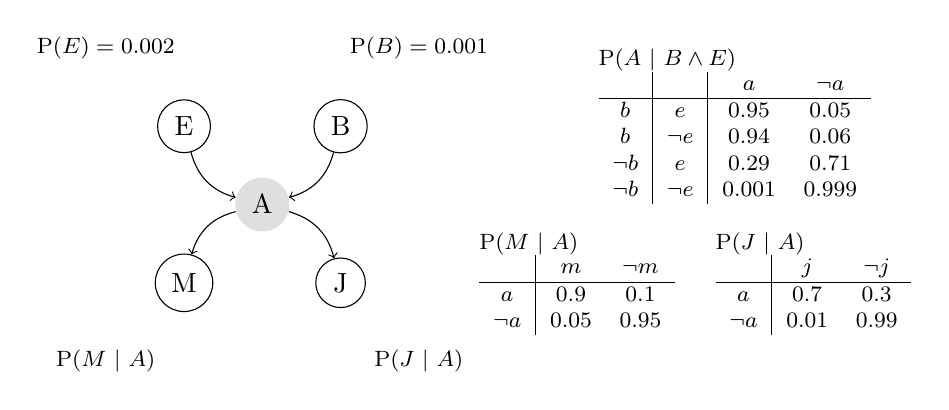
\begin{tikzpicture}[node distance=4em]

			% Nodes
			\node[smodel, circle] (A) {A}; \node[tchoice, above left of=A] (E)
			{E}; \node[above left of=E] {\footnotesize{\(\pr{E}=0.002\)}} ;
			\node[tchoice, above right of=A] (B) {B}; \node[above right of=B]
			{\footnotesize{\(\pr{B}=0.001\)}} ; \node[tchoice, below left of=A]
			(M) {M}; \node[below left of=M] {\footnotesize{\(\pr{M \given A}\)}}
			; \node[tchoice, below right of=A] (J) {J}; \node[below right of=J]
			{\footnotesize{\(\pr{J \given A}\)}} ;

			% Edges
			\draw[->] (B) to[bend left] (A); \draw[->] (E) to[bend right] (A);
			\draw[->] (A) to[bend right] (M) ; \draw[->] (A) to[bend left] (J);

			%   EDIT: fc Tables
			\node at (4,-1) {\footnotesize
				$
					\begin{aligned}
						 & \pr{M \given A}                   \\[-0.55em]
						 & \begin{array}{c|cc}
							            & m    & \neg m \\
							   \hline a & 0.9  & 0.1    \\
							   \neg a   & 0.05 & 0.95\end{array}
					\end{aligned}
				$};
			\node at (7,-1) {\footnotesize
				$
					\begin{aligned}
						 & \pr{J \given A}                   \\[-0.55em]
						 & \begin{array}{c|cc}
							            & j    & \neg j \\
							   \hline a & 0.7  & 0.3    \\
							   \neg a   & 0.01 & 0.99\end{array}
					\end{aligned}
				$};
			\node at (6,1) {\footnotesize
				$
					\begin{aligned}
						 & \pr{A \given B \wedge E}                     \\[-0.55em]
						 & \begin{array}{c|c|cc}
							            &        & a     & \neg a \\
							   \hline b & e      & 0.95  & 0.05   \\
							   b        & \neg e & 0.94  & 0.06   \\
							   \neg b   & e      & 0.29  & 0.71   \\
							   \neg b   & \neg e & 0.001 & 0.999\end{array}
					\end{aligned}
				$};

		\end{tikzpicture}
	\end{center}
	\caption{The Earthquake, Burglary, Alarm model}
	\label{figure:bea.model}
\end{figure*}

We follow the convention of representing the (upper case) random
variable \(X\) by the (lower case) positive literal \(x\).
%
Considering the probabilities given in \cref{figure:bea.model} we obtain
the following specification:

\begin{equation*}
	\begin{aligned}
		\probfact{b}{0.001} & ,\cr \probfact{e}{0.002} & ,\cr \end{aligned}
	\label{eq:not_so_simple_example}
\end{equation*}

For the table giving the probability \(\pr{M \given A}\) we obtain the
program:

\begin{equation*}
	\begin{aligned}
		\probfact{\condsymb{m}{a}}{0.9} & ,\cr \probfact{\condsymb{m}{\co{a}}}{0.05} & ,\cr m & \clause a \wedge \condsymb{m}{a},\cr m & \clause \neg a \wedge \condsymb{m}{\co{a}}.
	\end{aligned}
\end{equation*}

The latter program can be simplified (abusing notation) by writing
\(\probrule{m}{0.9}{a}\) and \(\probrule{m}{0.05}{\co{a}}\).

Similarly, for the probability \(\pr{J \given A}\) we obtain
\begin{equation*}
	\begin{aligned}
		\probrule{j}{0.7}{  & a},      \\
		\probrule{j}{0.01}{ & \neg a},
	\end{aligned}
\end{equation*}

Finally, for the probability \(\pr{A \given B \wedge E}\) we obtain
\begin{equation*}
	\begin{aligned}
		\probrule{a}{0.95}{b \wedge e},                                              &  &  &
		\probrule{a}{0.94}{b \wedge \co{e}},\cr \probrule{a}{0.29}{\co{b} \wedge e}, &  &  &
		\probrule{a}{0.001}{\co{b} \wedge \co{e}}.
	\end{aligned}\label{eq:prA.given.B.and.E}
\end{equation*}

One can then proceed as in the previous subsection and analyze this
example.  The details of such analysis are not given here since they
are analogous, albeit admittedly more cumbersome.

\bibpunct{(}{)}{;}{a}{}{;}
\bibliographystyle{kluwer}
\bibliography{zugzwang}

\end{document}
